\chapter{Algorytm rankingowy}

\section{Opis eksperymentów}

\subsection{Przygotowanie danych i symulacja}

W celu weryfikacji stworzonej przez nas koncepcji algorytmu rankingowego stworzona została aplikacja symulująca proces oceniania recenzji. Model danych aplikacji testowej jest uproszony względem systemu revCommunity i obejmuje tylko użytkowników i recenzje. 
Każdy z użytkowników posiada zbiór recenzji swojego autorstwa, liczbę recenzji które oceni w trakcie symulacji, a także wartość procentową określającą  domyślne prawdopodobieństwo otrzymania pozytywnego głosu przez recenzję jego autorstwa. Dodatkowo każdy z użytkowników może zostać oznaczony jako oszust, co spowoduje, że w trakcie głosowania będzie oceniał dobre recenzje jako złe i odwrotnie. Użytkownicy - oszuści mają za zadanie symulować obecnych w realnym świecie użytkowników sponsorowanych.
Recenzje posiadają natomiast unikatowy identyfikator, liczbę uzyskanych głosów pozytywnych i negatywnych, przydatność, autora, a także prawdopodobieństwo otrzymania pozytywnego głosu, które jest liczbą losową z zakresu [90\% x ; 110\% x], gdzie x to domyślne prawdopodobieństwo otrzymania pozytywnego głosu przypisane do autora recenzji. Należy dodatkowo zaznaczyć, że wylosowane prawdopodobieństwo jest zawsze liczbą z zakresu [0;1]
Ważną rolę w programie testowym odgrywają także parametry, pozwalające sterować przebiegiem symulacji. Wszystkie dostępne ustawienia deklarowane są w klasie AbstractParameters, z której dziedziczy klasa Parameters określająca domyślną wartość każdego parametru. Na jej podstawie budowane są kolejne zbiory parametrów przydatne dla poszczególnych testów, nadpisujące tylko niezbędne wartości. Najważniejsze parametry, które można dostosować w opisywanej aplikacji testowej to:

\begin{itemize}
\item Wagi oraz wartości stałe wykorzystywane podczas obliczania przydatności recenzji i oceny autora,
\item Liczba użytkowników biorących udział w symulacji,
\item Procentowy udział użytkowników - oszustów,
\item Liczba recenzji biorących udział w symulacji.
\end{itemize}


Wykonie symulacji wymaga wcześniejszego wygenerowania kolekcji użytkowników i recenzji. W celu lepszego odwzorowania rzeczywistości użytkownicy zostają podzieleni na trzy grupy:  przeciętnych, aktywnych i biernych. Użytkownikowi należącemu do odpowiedniej grupy przypisywana jest następnie liczba recenzji które oceni podczas symulacji. Średnia liczba recenzji przypadająca na użytkownika określana jest za pomocą stałej wartości ze zbioru parametrów i odpowiada ona liczbie recenzji ocenianych przez przeciętnych użytkowników. Użytkownicy aktywni mają natomiast przyporządkowaną losową wartość większą od średniej, a użytkownicy bierni mniejszą. Następnie, spośród wszystkich użytkowników losowana jest określona przez parametry liczba oszustów. Ostatnim elementem procesu jest wylosowanie użytkowników będących autorami recenzji. Każdemu z nich przyporządkowywane jest domyślne prawdopodobieństwo otrzymania pozytywnego głosu. Kolejnym etapem jest proces generowania recenzji, w którym każdej z nich przyporządkowywany jest losowy autor, a także losowane jest prawdopodobieństwo otrzymania pozytywnego głosu.

Po wygenerowaniu niezbędnych obiektów następuje symulacja oceniania recenzji przez użytkowników. Pierwszym etapem procesu jest wylosowanie dla każdego użytkownika określonej liczby recenzji, które oceni w czasie symulacji. Następnie, dla każdej z nich losowana jest wartość z zakresu [0;1], która jeśli okaże się większa lub równa prawdopodobieństwu otrzymania pozytywnego głosu powoduje zwiększenie licznika głosów negatywnych recenzji. W przeciwnym wypadku inkrementowany jest licznik głosów pozytywnych. Sytuacja wygląda inaczej jeżeli oceniający jest oszustem. Wtedy wylosowanie liczby większej niż przypisane recenzji prawdopodobieństwo skutkuje dodaniem głosu pozytywnego. 

Ostatecznie dla każdej recenzji wyliczana jest przydatność przy wykorzystaniu omówionego w rozdziale drugim wzoru i przygotowywany jest specyficzny dla danego testu raport.

\subsection{Test I - przegląd danych}

Pierwszy z przygotowanych przez nas testów umożliwia pełny podgląd systemu po przeprowadzeniu symulacji. Jego kod źródłowy znajduje się w klasie DefaultTest. Dzięki niemu możemy podejrzeć podstawowe informacje, takie jak wagi użyte do obliczania przydatności czy średnią użyteczność w systemie, ale również szczegółowe dane dotyczące recenzji i recenzentów. Dla recenzji są to kolejno:

\begin{itemize}
\item identyfikator,
\item prawdopodobieństwo otrzymania pozytywnego głosu, będąca jednocześnie oczekiwaną wartością przydatności,
\item liczbę oddanych głosów,
\item liczbę głosów pozytywnych,
\item stosunek głosów pozytywnych do wszystkich,
\item przydatność,
\item błąd czyli różnica między przydatnością oczekiwaną a uzyskaną, podniesiona do kwadratu.
\end{itemize}

Dane użytkowników reprezentowane są przez:

\begin{itemize}
\item identyfikator,
\item liczbę głosów oddanych na recenzje użytkownika,
\item liczbę głosów pozytywnych,
\item ocenę użytkownika,
\item identyfikatory recenzji należących do użytkownika.
\end{itemize}

Całkowity przegląd danych okazał się szczególnie przydatny w ustalaniu odpowiednich wag i wartości stałych biorących udział w obliczaniu przydatności recenzji i oceny autora.

Wartości błędów wykorzystane są do obliczenia RMSE (ang. root mean squared error), który pozwala na szybkie porównanie różnych przypadków testowych. RMSE mierzy o ile jednostek średnio różnią się wartości obliczone od wartości domyślnej.\cite{rmseWiki}\\

$ RMSE=\sqrt{\frac{\sum_{t=1}^n (\bar{y_{t}}-y_{t})^2}{n}} $\\\\
gdzie:\\
n- liczba pomiarów\\
$\bar{y_{t}}$ - wartość domyślna\\
$y_{t}$ - wartość uzyskana\\

\subsection{Test II - Badanie wpływu liczby głosów na błąd przydatności}

Kolejny test, którego źródło znajduje się w klasie ProgressiveTest, posłużył do zbadania zależności pomiędzy liczbą użytkowników, która przekłada się na liczbę oddanych głosów, a różnicą pomiędzy spodziewaną i uzyskaną wartością przydatności, wyrażoną w postaci RMSE. Intuicja podpowiada, że im więcej głosów oddano na recenzję, tym jej przydatność jest bardziej wiarygodna, a tym samym błąd powinien być mniejszy. Aby sprawdzić czy wspomniana zależność jest zachowana, przygotowaliśmy test, w którym symulacja powtarzana jest kilkakrotnie, za każdym razem z dla innej liczby użytkowników. Przed wykonaniem testu istnieje możliwość ustawienia początkowej i końcowej wartości tego parametru, a także wartość o jaką parametr ten będzie zwiększany w każdej iteracji. Liczba recenzji dla każdej iteracji pozostaje stała.


Poniżej przedstawiono raport uzyskany po wykonaniu testu dla 100 recenzji i wzrastającej liczby użytkowników z zakresu od 30 do 300. Nagłówek zawiera wartość stałą i wagi wykorzystane do obliczenia przydatności recenzji. Poniżej znajdują informacje o każdej z iteracji. Pierwsza kolumna informuje o liczbie użytkowników. Kolejna zawiera błąd w postaci RMSE, natomiast ostatnia średnią liczbę głosów przypadających na recenzję. Poniżej przedstawiono również wykres stworzony na podstawie raportu. Obrazuje on wpływ wzrostu liczby użytkowników na wartość RMSE.

\begin{lstlisting}
defaultUsefulnessWeight: 1
reviewRateWeight: 8
authorRateWeight: 3
const: 15

users	RMSE	votes/review	
30	0.05942	8.93
60	0.05217	12.83
90	0.04425	18.09
120	0.0424	24.76
150	0.04169	32.71
180	0.03963	40.35
210	0.03967	47.47
240	0.03859	55.32
270	0.03554	62.94
300	0.03585	70.78
\end{lstlisting}

\begin{figure}[h]
	\centering
	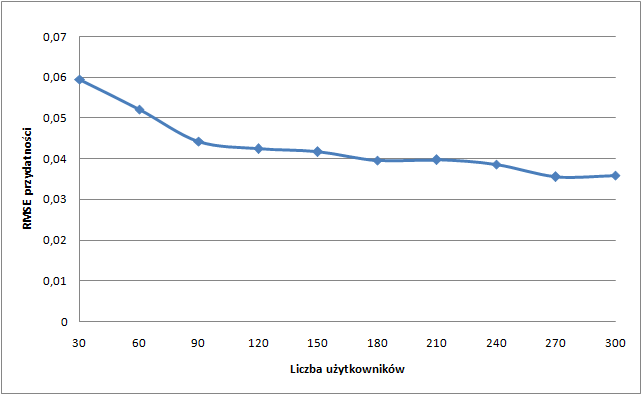
\includegraphics[scale=0.7]{images/ProgressiveTest.png}
	\caption{Liczba użytkowników a pierwiastek błędu średniokwadratowego przydatności recenzji}
\end{figure}

Analizując uzyskane dane, można zauważyć, że wzrost liczby użytkowników, a co za tym idzie, głosów oddanych na recenzje, istotnie powoduje spadek błędu. Innymi słowy, recenzje posiadające więcej głosów posiadają użyteczność bliższą wartości oczekiwanej. Dzieje się tak, ponieważ wraz ze wzrostem liczby głosów oddanych na recenzję, rośnie ich wpływ na wartość wyliczanej użyteczności. Dla małej liczby głosów, użyteczność recenzji normalizowana jest przez wartość domyślnej użyteczności.

\subsection{Test III - Badanie odporności systemu na obecność użytkowników - oszustów}

Ostatni z testów dotyczy odporności systemu na obecność użytkowników - oszustów. Jego kod źródłowy znajduje się w pliku LiarsTest.java. Głównym celem testu jest sprawdzenie jak zmienia się wartość błędu wraz z wzrostem liczby kłamców w systemie. Podobnie jak w poprzednim teście, kolejne symulacje przeprowadzane są dla rosnącej liczby użytkowników, lecz dodatkowo także dla rosnącej liczby oszustów. Przedstawiony poniżej fragment raportu zbliżony jest do raportu z poprzedniego testu. W nagłówku drukowane są parametry średniej Bayesa, a następnie kolejno w kolumnach: udział procentowy oszustów, RMSE dla przydatności i średnia liczba głosów przypadająca na recenzję. Każda seria danych posiada także informację o liczbie użytkowników.

\begin{lstlisting}
defaultUsefulnessWeight: 1
reviewRateWeight: 8
authorRateWeight: 3
const: 15


liars%	RMSE	votes/review

users:	210
0	0.03803	39.59167
10	0.06425	40.025
20	0.12165	39.45833
30	0.16595	39.14167
40	0.22776	40.04167
50	0.26943	40.64167
\end{lstlisting}

Poniżej przedstawiony został wykres ukazujący wpływ ilości kłamców na wartość RMSE dla przydatności. Na osi rzędnych znajdują się wartości RMSE przydatności, natomiast na osi odciętych liczba użytkowników. Poszczególne serie danych dotyczą innej wartości procentowego udziału oszustów i zostały oznaczone kolorami. Liczba recenzji jest stała i wynosi 120.

\begin{figure}[h]
	\centering
	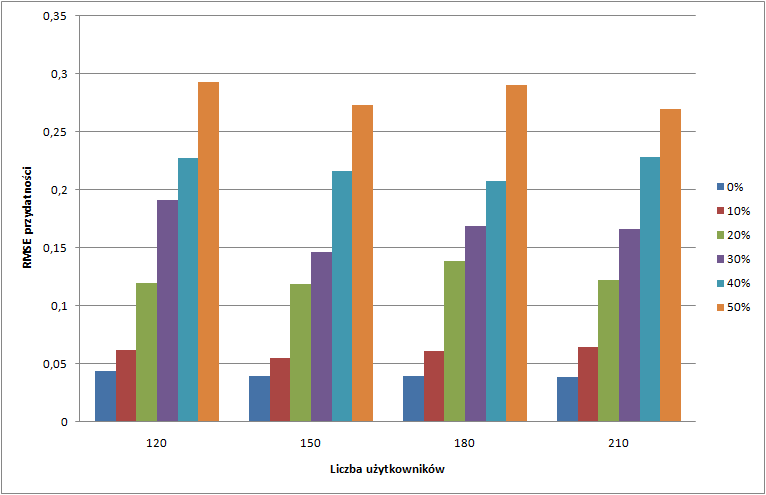
\includegraphics[scale=0.7]{images/LiarsTest.png}
	\caption{Liczba użytkowników a pierwiastek błędu średniokwadratowego przydatności recenzji}
\end{figure}

Jak widać na powyższym wykresie, wzrost liczby oszustów w systemie skutkuje wzrostem wartości błędu niezależnie od liczby użytkowników. Ponadto, warto zauważyć, że przy dziesięcioprocentowym udziale oszustów w systemie wartość błędu różni się nieznacznie od wartości błędu w sytuacji gdy wszyscy użytkownicy są rzetelni.

\section{Implementacja}

W celu implementacji algorytmu rankingowego stworzone zostały metody pozwalające obliczyć przydatność recenzji i ocenę recenzenta, a także metody pomocnicze obliczające ich składowe. Przydatność recenzji oraz ocena autora zrealizowane zostały jako pola, odpowiednio w klasach Review i User, których obiekty przechowywane są w bazie danych. Umożliwiło nam to przede wszystkim efektywne sortowanie danych na poziomie bazy danych. Wspomniane wartości obliczane są za każdym razem gdy któryś z użytkowników odda głos na recenzję. Część kliencka aplikacji rozpoczyna wtedy asynchroniczną komunikację z serwerem i wysyła informację o typie głosu, identyfikatorze recenzji i nazwie użytkownika, który ten  głos oddał. Na serwerze, dane przetwarzane są w ramach jednej transakcji dzięki czemu zachowana jest ich spójność \cite{springAction}. Głos zostaje skojarzony z zalogowanym użytkownikiem i ocenioną recenzją, a następnie obliczana jest nowa wartość użyteczności recenzji i rangi jej autora. Wartości te są następnie przesyłane do warstwy klienckiej i  prezentowane użytkownikowi.

Jednym z elementów potrzebnych do obliczenia przydatności recenzji jest średnia przydatność wszystkich recenzji w systemie. W przypadku bardzo dużej bazy danych obliczenie tej wartości byłoby bardzo czasochłonne, a to spowodowałoby znaczny wzrost czasu odpowiedzi serwisu. Aby temu zapobiec, postanowiliśmy przechowywać aktualną wartość średniej w bazie danych i aktualizować ją okresowo przy wykorzystaniu biblioteki Quartz, która umożliwia wykonywanie zadań w określonych odstępach czasu bez interakcji z użytkownikiem.\cite{quartz} Każdorazowe przeliczenie średniej wiąże się dodatkowo z przeliczeniem przydatności dla każdej recenzji, tak by odzwierciedlały aktualny stan systemu i można było je porównywać. Oczywiście, takie rozwiązanie najlepiej sprawdza się w przypadku gdy liczba  recenzji w bazie jest stosunkowo duża, ponieważ można wtedy założyć, że pojedynczy głos ma bardzo mały wpływ na średnią i jej ciągłe przeliczanie byłoby nieopłacalne.

\section{Problemy i wnioski}

Przedstawiona koncepcja algorytmu rankingowego może być z powodzeniem zastosowana w komercyjnym serwisie. Dzięki zastosowaniu średniej Bayesa, system daje użytkownikowi możliwość zaobserwowania nie tylko jak dany produkt jest oceniany ale także jak wypada na tle innych produktów. Dodatkowo, ranking zbudowany przy zastosowaniu proponowanej koncepcji jest bardziej wiarygodny i odporny na manipulację przez nieuczciwych użytkowników.

Proponowane rozwiązanie niesie ze sobą także pewne problemy. Najważniejszym z nich jest dobór stałych wykorzystywanych we wzorach na przydatność i rangę użytkownika. Wartości te dobierane są w oparciu o intuicję lub eksperymentalnie, co niesie ryzyko, że wybrana ostatecznie konfiguracja okaże się nieoptymalna.
